
\newpage
\thispagestyle{empty}
\mbox{}
\chapter{Sistema de manera global}
\label{ch:chapter2}

\section{Algoritmo de estimación de búsqueda de fuentes} \label{Estima}

Anteriormente se discutió que el objetivo del algoritmo es la búsqueda de fuentes, basándose en mediciones locales de múltiples robots situados de manera simétrica en un espacio de 2D. En dicho procedimiento, se consideran N robots distribuidos uniformemente a lo largo de una formación circular con un radio D y un punto central c definido en dos dimensiones, tal como se muestra en la siguiente figura: \\

\begin{figure}[htb]
\centering
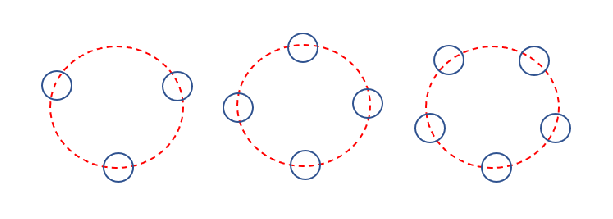
\includegraphics[width=0.95\textwidth]{figures/Disposicion_Robots.eps}
\caption{Disposición de los agentes en torno a la formación circular.} \label{Disp:Robots}
\end{figure}
\newpage
Adicionalmente, cada uno de los agentes deberá tener la capacidad de medir la intensidad de la señal mediante un sensor. En términos matemáticos, la distribución de la señal es una función espacial bidimensional que representa un campo escalar con un máximo o mínimo definido justo en la posición donde dicha fuente se localiza. Por lo tanto, se va a considerar que la señal es emitida por una única fuente de modo que su punto de inflexión en $z_*$ es el único máximo definido del campo escalar.

Para dicho calculo, adopta vital importancia los \textbf{algoritmos de tipo consenso} siendo estos un mecanismo que permite a maquinas coordinarse en un entorno distribuido, es decir, encuentran la solución al problema de la comunicación entre diferentes entes aislados con el objetivo de ponerse de acuerdo para realizar una tarea concreta.

Por lo tanto, se define una función $f\left(x\right)$ con $x\in\mathbb{R}^{n}$, además de ser continua y derivable para todo n. Aplicando el desarrollo en serie de Taylor para un valor de $n\geq{2}$ se tiene:

\begin{equation}\label{TaylorNormal}
	f\left(x\right)=f\left(x_{*}\right)+\mathrm{\nabla}{f}{\left(x_{*}\right)}^{T}\left(x-x_{*}\right)+\frac{1}{2!}\cdot{\left(x-x_{*}\right)}^{T}\cdot{H}\left({f}\left(x_{*}\right)\right) 		\cdot\left(x-x_{*}\right)+O\left(x_{*}^3\right)
\end{equation}

Donde:

\begin{equation*}
	\begin{aligned}
		\mathrm{\nabla}{f}=
	\begin{bmatrix}
		\frac{\partial{f}}{\partial{x}_1} \\
		\frac{\partial{f}}{\partial{x}_2}  \\
		\vdots \\
		\frac{\partial{f}}{\partial{x}_n}
	\end{bmatrix}
	\end{aligned}
	\qquad\text{y}\qquad
	\begin{aligned}
	{H}\left(f\right)=\mathrm{\nabla}^{2}{f}= 	
	\begin{bmatrix}
		\frac{\partial^{2}{f}}{\partial{x}_{1}^{2}} & \frac{\partial^{2}{f}}{\partial{x}_{1}\cdot\partial{x}_{2}} & \cdots & \frac{\partial^{2}{f}}{\partial{x}_{1}\cdot\partial{x}_{n}}\\
		\frac{\partial^{2}{f}}{\partial{x}_{2}\cdot\partial{x}_{1}} & \frac{\partial^{2}{f}}{\partial{x}_{2}^{2}} & \cdots & \frac{\partial^{2}{f}}{\partial{x}_{2}\cdot\partial{x}_{n}}\\
		\vdots & \vdots & \ddots & \vdots\\
		\frac{\partial^{2}{f}}{\partial{x}_{n}\cdot\partial{x}_{1}} & \frac{\partial^{2}{f}}{\partial{x}_{n}\cdot\partial{x}_{2}} & \cdots & \frac{\partial^{2}{f}}{\partial{x}_{n}^{2}}
	\end{bmatrix}
	\end{aligned}
\end{equation*}

Para evaluar el punto máximo de concentración lo que interesa es que $\mathrm{\nabla}{f}{\left(x_{*}\right)}=0$. No obstante, en el problema en cuestión no se dispone de información sobre dicho gradiente solo se tienen las medidas tomadas por los sensores en cada uno de los vehículos es por ello que se va a aprovechar la simetría existente para realizar una estimación del gradiente $\hat{\nabla}{f}\left(c\right)$


\begin{figure}[htb]
\centering
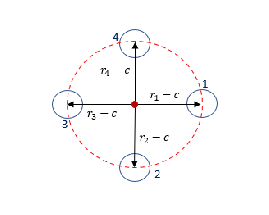
\includegraphics[width=0.5\textwidth]{figures/p3.eps}
\caption{Estrategia colaborativa para la búsqueda de fuentes.} \label{Estrategia_Colaborativa}
\end{figure}

Particularizando para una distribución uniforme a lo largo de un circulo con radio D, un ángulo de rotación $\phi_o\left(t\right)=w_ot$ y el centro de la formación c. 

\begin{equation*}
	r_i = c + D\cdot{R}_{\theta_i}\cdot{e}\hspace{10mm}{i = 1,...,N}
\end{equation*}

En donde, $r_{i}$ es la posición del robot i con respecto al radio del circulo, ${\phi }_{i}=\phi_o\frac{2\cdot\pi\cdot{i}}{N}$ es el ángulo de rotación, $R_{\phi }$ es la matriz de rotación definida como $\left[ \begin{array}{cc} {c}_{\phi } & -{s}_{\phi } \\  {s}_{\phi } & {c}_{\phi } \end{array} \right]$ y  $e\ =\ {\left[1,0\right]}^T$.\\


A partir de la ecuación \ref{TaylorNormal} pero haciendo la expansión de Taylor hasta el termino primer orden sobre cada una de las medidas $f\left(r_i\right)$ en torno al punto c y redefiniendo a $D$ como $D=||r_i-c||$, se obtiene:

\begin{equation} \label{PuntoPartidaGradiente}
	f\left(r_i\right)-f\left(c\right)=\nabla{f\left(c\right)}^T\left(r_i-c\right)+\varphi_i\left(D,c\right)\hspace{12mm}\forall{i},\cdots,N
\end{equation}

En donde, $\varphi_i\left(D,c\right)$ denota el remanente de la expansión de Taylor. 
\newpage
Cabe destacar que la anterior ecuación no se va a utilizar directamente dado que en lugar de evaluar el valor de la función según su gradiente conocido se realiza el proceso inverso, es decir, en función de las distintas medidas tomadas por los vehículos se estimará el gradiente el cual se encuentra definido en el centro de la formación circular. Por ende, la ecuación \ref{PuntoPartidaGradiente} se multiplica por $\left(\frac{2}{ND^{2}}\right)\left(r_i-c\right)$ y se hace el sumatorio en torno a $i=1,\cdots,N$, obteniéndose:

\begin{equation}\label{Fun_Esti}
	\frac{2}{N\cdot{D}^2}\cdot\sum_{i=1}^{N}f(r_{i})\cdot(r_{i}-c)=\underbrace{\nabla{f}\left(c\right) + \varphi\left(D,c\right)}_{:=\hat{\nabla}{f}\left(c\right)}
\end{equation}

En donde, $\varphi\left(D,c\right)$ es el error de la aproximación. Adicionalmente, para evaluar la dependencia de la estima con respecto al número de agentes dispuestos en la formación y a su vez del radio de esta, se define a la función gaussiana de la figura \ref{FunGauss} como:

\begin{equation}\label{Gaussiana_base}
	f\left(x\right)=\frac{1}{\sigma\sqrt{2\pi}}e^{\frac{\left(x-\mu\right)^2}{2\sigma^2}}\hspace{12mm}con\hspace{1mm}x\in\mathbb{R}^{2}
\end{equation}

En donde, $\sigma$ es la desviación típica aportando información sobre la variación de la concentración de las sustancias y $\mu$ la media que representa el punto de máxima radiación de la fuente. Un aspecto relevante es que si el centro de la formación se encuentra lo suficientemente cerca de la fuente el argumento de la exponencial tenderá a 0 conllevando a que en torno a dicho punto se tenga la máxima concentración de sustancias.

Posteriormente, se establece una posición arbitraria para el centro de la formación que se encuentre relativamente lejos de la fuente para poder evaluar la variación del número de agentes con un radio unitario y del radio con el mínimo de número de agentes posibles.

\newpage
\begin{figure}[htb]
  \begin{center}
    \subfigure[N = 2]{
        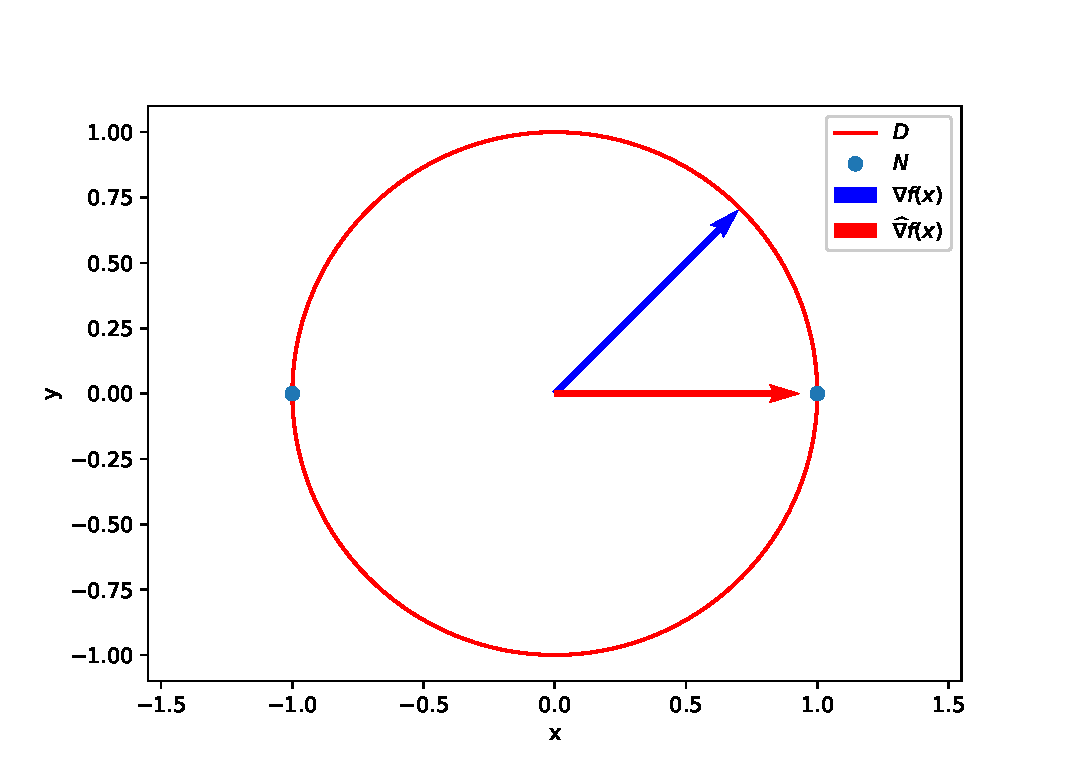
\includegraphics[width=0.40\textwidth]{figures/N2_RFIJO.eps}
        \label{N = 2}}
    \subfigure[N = 3]{
        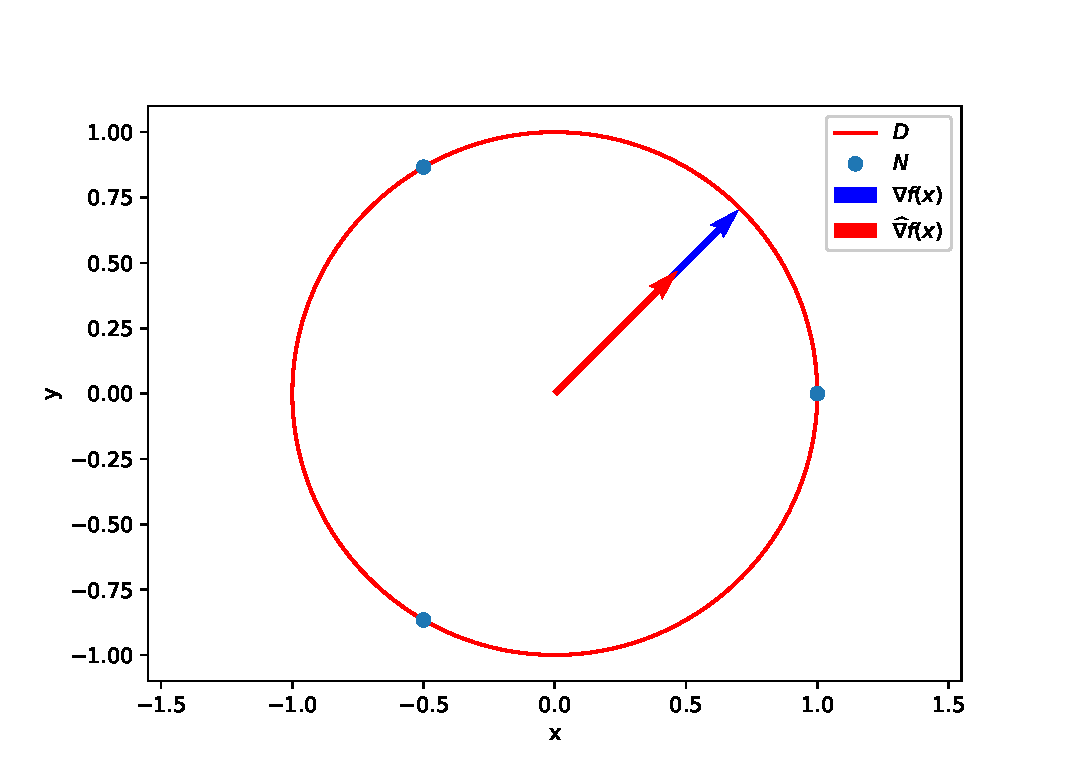
\includegraphics[width=0.40\textwidth]{figures/N3_RFIJO.eps}
        \label{N = 3}}
    \caption{Estimación del gradiente en función del número de agentes}
    \label{NAGENTSEST}
  \end{center}
\end{figure}

Se observa en la figura que al aumentar el número de agentes llega un punto donde el error es prácticamente despreciable, además de que con dos vehículos es absurdo obtener una estimación del gradiente es por ello, tal como se anticipaba en [referencia bibliografica], que el algoritmo funciona siempre y cuando sean 3 o más vehículos. De manera análoga, se procede a evaluar el efecto del radio:

\begin{figure}[htb]
  \begin{center}
    \subfigure[D = 100]{
        \includegraphics[width=0.40\textwidth]{figures/R100_NFIJO.eps}
        \label{D = 100}}
    \subfigure[D = 10]{
        \includegraphics[width=0.40\textwidth]{figures/R10_NFIJO.eps}
        \label{D = 10}}
    \caption{Estimación del gradiente en función del radio del círculo}
    \label{VARD}
  \end{center}
\end{figure}

En este caso la relación es inversa al número de agentes, es decir, entre menor sea el radio menor será el error. No obstante, se debe de tener en cuenta las dimensiones de los vehículos dado que si el radio es excesivamente pequeño pueden generarse colisiones entre ellos.

Finalmente, en los capítulos posteriores se hará un estudio más detallado del resto de parámetros y sus respectivos efectos sobre la búsqueda de fuentes. Más concretamente, se estudiará cuando el sistema este definido de manera global, antes se debe discutir la importancia que tiene la coordinación de los agentes en torno a la formación circular.

\section{Algoritmo de control de formación circular}

El control de la formación tiene como objetivo evaluar la cooperación y la coordinación en sistemas con múltiples agente, donde su uso recae en impulsarlos a lograr unas restricciones prescritas en sus estados conllevando a formar y mantener una forma geométrica deseada.

\begin{figure}[htb]
\centering
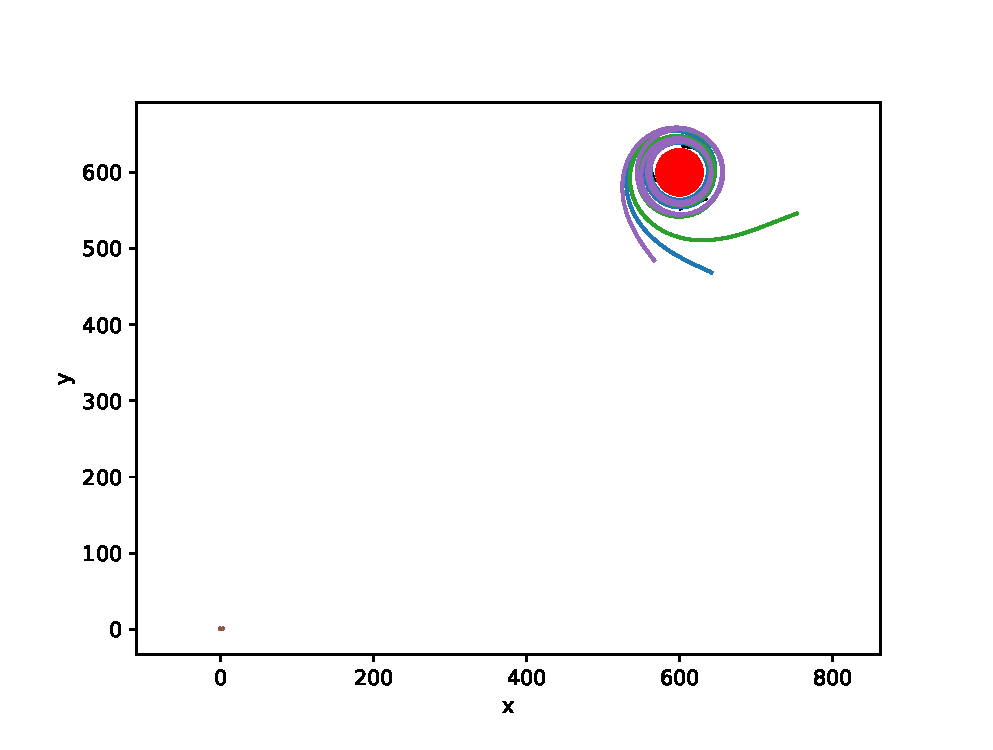
\includegraphics[width=0.90\textwidth]{figures/Coordinacion/Objetivo_Final.eps}
\caption{Vehículos dispuestos en torno a la formación. El punto rojo representa el circulo al que quieren converger y los diferentes colores que girar en torno a dicho punto son cada uno de los vehículos.} \label{Ejemplo_Coordinacion}
\end{figure}
\newpage

El problema de control que se utilizará considera vehículos tipo monociclo con velocidad constante, es decir, solo se actúa sobre la dirección del vehículo a través de giros coordinados actuando sobre el ángulo de inclinación lateral. Definiéndose como objetivo el describir un \textbf{algoritmo distribuido para controlar formaciones circulares} aplicados a los USVs comentados en \ref{Motiv}. Estos tendrán velocidades constantes y se actuará sobre el radio del circulo a ser rastreado no sobre la dirección de cada uno de los agentes, es decir, altera la velocidad angular que poseen en torno a un punto central. 

Es importante destacar que el algoritmo va a tener dos tareas:

\begin{itemize}
	\item Inicialmente cada uno de los vehículos estarán en posiciones arbitrarias y deberán converger hacia la formación circular definida en torno a un punto central conocido.
	\item Posteriormente, han de disponerse de manera simétrica en torno a dicha formación. Esto será posible al minimizar el error existente entre sus ángulos como más adelante se comentará.
\end{itemize}

No obstante, para ambos casos se tiene que tomar en cuenta la manera de comunicarse entre los agentes que se describe a continuación. 

Inicialmente, se considera una formación con $N\geq{2}$ USVs cuyas posiciones $p$ se definen por $p_i\in\mathbb{R}^2$ con $i\in\left\lbrace{1,\cdots,N}\right\rbrace$, en donde los vehículos son capaces de detectar las posiciones relativas con respecto a sus vecinos. Evaluando la relación existente entre los vecinos con respecto a su disposición en el plano puedes apreciar que forman un grafo $\mathbb{G}=\left(\mathcal{V},\mathcal{E}\right)$ siendo $\mathcal{V}=\left\langle{1,\cdots,N}\right\rbrace$ los distintos nodos pertenecientes al grafo y  $\mathcal{E}\subseteq\mathcal{V}\times\mathcal{V}$. El conjunto de los vecinos del vehículo $i$ esta definido por $\mathcal{N}_i\triangleq\left\lbrace{j\in\mathcal{V}:\left(i,j\right)\in\mathcal{E}}\right\rbrace$. Dos vértices son adyacentes si $\left(i,j\right)\in\mathcal{E}$. Un camino desde el nodo $i$ hasta el nodo $j$ es una secuencia que comienza en $i$ y termina en $j$, de manera que dos vértices consecutivos son adyacentes, y si $i=j$ el camino se le conoce como ciclo. \cite{Control_Formacion}

Asumiendo que el grafo $\mathbb{G}$ esta conectado, es decir existe un camino para cada par de nodos $i$ y $j$. Se definen los elementos de la matriz de incidencia $B\in\mathbb{R}^{|\mathcal{V}|\times|\mathcal{V}|}$, donde $|\chi|$ representa la cardinalidad del conjunto $\chi$, para $\mathbb{G}$ dado por:

\begin{equation} \label{Incidence}
  b_{ik}\triangleq\left \{
    \begin{aligned}
+1\hspace{5mm}si\hspace{5mm}i&=\mathcal{E}^{cola}_{k}\\
-1\hspace{5mm}si\hspace{5mm}i&=\mathcal{E}^{cabeza}_{k}\\
0\hspace{5mm}Cualquier\hspace{1mm}otro\hspace{1mm}caso
    \end{aligned}
  \right .
\end{equation}

En donde $\mathcal{E}^{cola}_{k}$ y $\mathcal{E}^{cabeza}_{k}$ representa los nodos cola y cabeza de la arista $\mathcal{E}_{k}$, es decir, $\mathcal{E}_{k}=\left(\mathcal{E}^{cola}_{k},\mathcal{E}^{cabeza}_{k}\right)$. Un ejemplo de esto puede observarse en la figura \ref{Estrategia_Colaborativa} en el que se tienen 4 vehículos conformando un grafo en si mismo, en donde, el 1 puede pasarle la información sobre su posición al 4 y 2, el 2 con el 1 y 3, y así sucesivamente.

Posteriormente, se debe definir una trayectoria circular de radio $D\in\mathbb{R}^+$ puede ser descrita mediante la siguiente ecuación:

\begin{equation}
	C_D\triangleq\left\lbrace{p:\varphi{\left(p\right)}=0}\right\rbrace{,}
\end{equation}

En donde, $\varphi{p}=p_{x}^{2}+p_{y}^{2}$ y $p=\left[p_x\hspace{2mm}p_y\right]^T$ que representa la posición cartesiana con respecto a un marco de coordenadas cuyo origen esta en el centro de $C_D$. El plano $\mathbb{R}^2$ puede cubrirse con los siguientes conjuntos disjuntos $\varphi_c\left(p\right)\triangleq\varphi\left(p\right)=c\in\mathbb{R}$, donde cada conjunto de niveles se define para un valor particular $c$ tal que el radio del circulo resultante no es negativo y, en particular, el conjunto de niveles cero corresponde únicamente a $C_D$ \cite{Control_Formacion}, además $C_D$ pertenece al espacio $\mathbb{C}^2$ y este es regular para cualquier posición exceptuando en el centro, es decir, $\nabla{\varphi\left(p\right)}\neq{0}\Longleftrightarrow{p}\neq{0}$ y todo el conjunto de niveles $\varphi_c\left(p\right)$ se puede parametrizar. 
\newpage
\begin{figure}[htb]
\centering
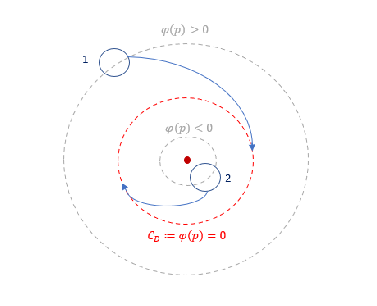
\includegraphics[width=0.60\textwidth]{figures/Pruea_Coordinacion.eps}
\caption{Ejemplo del algoritmo de control de formación} \label{Ejemplo_Coordinacion}
\end{figure}

Por ende, si se considera que la velocidad unitaria del vehículo se rastrea correctamente, por lo tanto su velocidad angular en torno al centro de $C_D$ esta definida como:

\begin{equation}
	\dot{\theta}_i=\frac{1}{r}
\end{equation}

La idea es controlar el ángulo entre vehículos $z = B^{T}\theta$ modificando la trayectoria descrita por cada uno y haciéndolos converger a la formación circular deseada. Cabe destacar que el valor de $\theta$ en la ecuación antes comentada equivale a $atan2(p_y,p_x)\in\left(-\pi,\pi\right]$ para cada una de las posiciones definidas en el plano. Se define:

\begin{equation}\label{Control}
	C_i\left(D,c_{i}\right)\triangleq\left\lbrace{p:\varphi\left(p\right)=c_{i}}\right\rbrace
\end{equation}

En donde, $c_i \in \mathbb{R}$ siendo la señal de control de formación y el subindice $i\in\mathcal{V}$ denota cada uno de los vehículos. A partir de dicha ecuación surgen dos situaciones:
\newpage

\begin{itemize}
	\item Si $c_i$ se hace muy pequeño, el radio D tenderá a aumentar y con ello se reduce la velocidad angular $\dot{\theta}_i$. Situación del agente 1 en la figura \ref{Ejemplo_Coordinacion}
	\item Si $c_i$ se hace muy grande, el radio D tenderá a disminuir y con ello se aumenta la velocidad angular $\dot{\theta}_i$. Situación del agente 2 en la figura \ref{Ejemplo_Coordinacion}
\end{itemize}

Se define a $c_i\triangleq{^{i}u}_{D}^{2}+2D\cdot{^i}u_{D},$ donde $^{i}u_{D}\in\mathbb{R}$ es una acción de control que posee un significado físico más directo al estar directamente imponiendo el radio de la circunferencia de la siguiente forma:

\begin{equation}
	x^2+y^2-r^2={^{i}}u_{D}^{2}+2D{^{i}}u_{D} \Leftrightarrow x^2+y^2-(r+{^{i}}u_{D})^2
\end{equation}

La acción de control adquiere el siguiente significado ${^{i}}{u}_{D}=k_{r}\sum_{i=1}^N{B_i}\cdot{e}$, definiendo a $B_i$ como cada una de las filas de la matriz de incidencia \ref{Incidence}, $k_r$ una constante $\in\mathbb{R}^{+}$ y $e$ se corresponde con el error de formación descrito como $e_{\theta_{k}}\left(t\right)=z_k\left(t\right)-z_{k}^*$, donde $e_{\theta_{k}}\in\left(-\pi,\pi\right]$ con $k\in\left\lbrace{1,\cdots,|\mathcal{E}|}\right\rbrace$. Definiendo como objetivo final del algoritmo que cuando $t\rightarrow\infty$ se tenga que $e_{\theta}\rightarrow{0}$ y $p_{i}\left(t\right)\rightarrow{C_D}$, en otras palabras, que pasado un tiempo el error sea el mínimo posible y a su vez cada uno de los vehículos este en la formación circular.

\section{Algoritmo de ascenso de gradiente}

Hasta el momento únicamente se ha comentado sobre la cooperación de los agentes para la disposición de una figura geométrica y simétrica requerida o un algoritmo para la localización de fuentes en el espacio. No obstante, se ha dejado de lado el avance de los agentes, es decir, ha de existir un algoritmo que desplace a todo el enjambre hacia la ubicación de la fuente haciendo uso del gradiente estimado.
\newpage
Para ello, se utiliza el algoritmo de ascenso de gradiente su objetivo principal es desplazar el centro de la formación circular dado que sobre este se encuentra definido el gradiente, la ecuación que lo describe presenta la siguiente forma \cite{Adicional_Estimacion_1}:

\begin{equation}\label{GA}
	c_{k+1}=c_k+\epsilon\nabla{f}\left(c_k\right)\hspace{10mm}c_k=[x,y]\hspace{2mm}\forall_{x,y}\in\mathbb{R}
\end{equation}

En donde, $c_k$ corresponde con el centro de la formación circular. Al tratarse de un problema definido como un punto máximo de una función, el avance ha de ser estrictamente positivo, es decir, los valores han de ser cada vez mayores para desplazarte hacia dicho punto.

\section{Operación conjunta de los tres algoritmos}

\begin{figure}[htb]
\centering
\includegraphics[width=0.55\textwidth]{figures/Flujo2.eps}
\caption{Diagrama de flujo que describe la dinámica del sistema.} \label{fig:Flujo}
\end{figure}

En la figura \ref{fig:Flujo} se pueden apreciar diferentes colores para diferenciar cada uno de los pasos a seguir antes de que los USVs lleguen a la zona con máximas sustancias contaminantes, desglosándolos estos serían:

\begin{enumerate}
	\item Se disponen los N agentes en el plano, es decir, se conoce la posición de cada uno de los USV en la superficie marítima.
	\item Se ejecuta el algoritmo de control de formación circular para hacer que convergan cada uno de los vehículos a la formación circular y a su vez se dispongan de manera simétrica. Un aspecto a destacar es que se tiene que poner un umbral para decidir cuando avanzar. Dicho umbral esta estrictamente relacionado con el error de la formación, es decir, si este valor es lo suficientemente pequeño el enjambre avanza; en caso contrario, se quedarán esperando a que todos los agentes se coloquen en sus sitios. 
	\item Al ya estar repartidos alrededor de la formación circular, se hace la estimación del gradiente para obtener la localización de las sustancias que en el algoritmo representa una fuente de radiación definida como máximo. En este punto, se dan dos casos que en la figura \ref{fig:Flujo} están referidos como A:
	\begin{itemize}
		\item Si $\widehat{\mathrm{\nabla }}{f}\left(c_{k}\right)\approxeq0$ se está cerca de la fuente conformando una \textbf{solución satisfactoria}.
		\item Si $\widehat{\mathrm{\nabla }}{f}\left(c_{k}\right)>0$ aun están desplazándose para llegar al objetivo.
	\end{itemize}
	\item En caso de darse la segunda de las situaciones antes planteadas, se ha de desplazar el centro de la formación circular mediante el algoritmo de ascenso de gradiente mediante la ecuación \ref{GA}.
	\item Antes de volver a estimar el gradiente se debe comprobar el paso 2, en caso de permanecer cada uno de los agentes en la formación y el error es lo suficientemente pequeño, se pasa directamente al paso 3.
\end{enumerate}








